\section{DUNE}
{{\footnotesize
\begin{description}[labelwidth=5em, labelsep=1em, leftmargin=*, align=left, itemsep=0.3em, parsep=0em]
  \item[date:] 2024-10-15
  \item[version:] TODO
  \item[last\_updated:] 2024-10
  \item[expired:] unknown
  \item[valid:] yes
  \item[valid\_date:] TODO
  \item[url:] \href{https://indico.fnal.gov/event/66520/contributions/301423/attachments/182439/250508/fast\_ml\_dunedaq\_sonic\_10\_15\_24.pdf}{https://indico.fnal.gov/event/66520/contributions/301423/attachments/182439/250508/fast\_ml\_dunedaq\_sonic\_10\_15\_24.pdf}
  \item[doi:] TODO
  \item[domain:] Particle Physics
  \item[focus:] Real-time ML for DUNE DAQ time-series data
  \item[keywords:]
    - DUNE
    - time-series
    - real-time
    - trigger
  \item[summary:] Applying real-time ML methods to time-series data from DUNE detectors, exploring trigger-level anomaly detection and event selection with low latency constraints.

  \item[licensing:] TODO
  \item[task\_types:]
    - Trigger selection
    - Time-series anomaly detection
  \item[ai\_capability\_measured:]
    - Low-latency event detection
  \item[metrics:]
    - Detection efficiency
    - Latency
  \item[models:]
    - CNN
    - LSTM (planned)
  \item[ml\_motif:]
    - Real-time, Time-series
  \item[type:] Benchmark (in progress)
  \item[ml\_task:]
    - Supervised Learning
  \item[solutions:] TODO
  \item[notes:] Prototype models demonstrated on SONIC platform

  \item[contact.name:] Andrew J. Morgan
  \item[contact.email:] unknown
  \item[datasets.links.name:] DUNE SONIC data
  \item[results.links.name:] ChatGPT LLM
  \item[fair.reproducible:] in progress
  \item[fair.benchmark\_ready:] False
  \item[ratings.software.rating:] 0
  \item[ratings.software.reason:] Not analyzed. 

  \item[ratings.specification.rating:] 8.0
  \item[ratings.specification.reason:] Task (quench detection via anomaly detection) is clearly described; multi-modal sensors, streaming rates, and objective are provided, but constraints (latency thresholds) are qualitative.

  \item[ratings.dataset.rating:] 7.0
  \item[ratings.dataset.reason:] Custom dataset using real data from BNL; HDF5 formatted and structured, but access may be internal or limited, and not versioned for public FAIR use.

  \item[ratings.metrics.rating:] 8.0
  \item[ratings.metrics.reason:] ROC-AUC and detection latency are defined; relevant and quantitative but not yet paired with benchmark baselines.

  \item[ratings.reference\_solution.rating:] 6.0
  \item[ratings.reference\_solution.reason:] Autoencoder prototype exists; RL methods are in development; no fully reproducible pipeline is available yet.

  \item[ratings.documentation.rating:] 7.0
  \item[ratings.documentation.reason:] Slides and GDocs outline results; implementation is in progress with limited setup/code release.

  \item[id:] dune
  \item[Citations:] \cite{abud2021deep}
  \item[Ratings:]
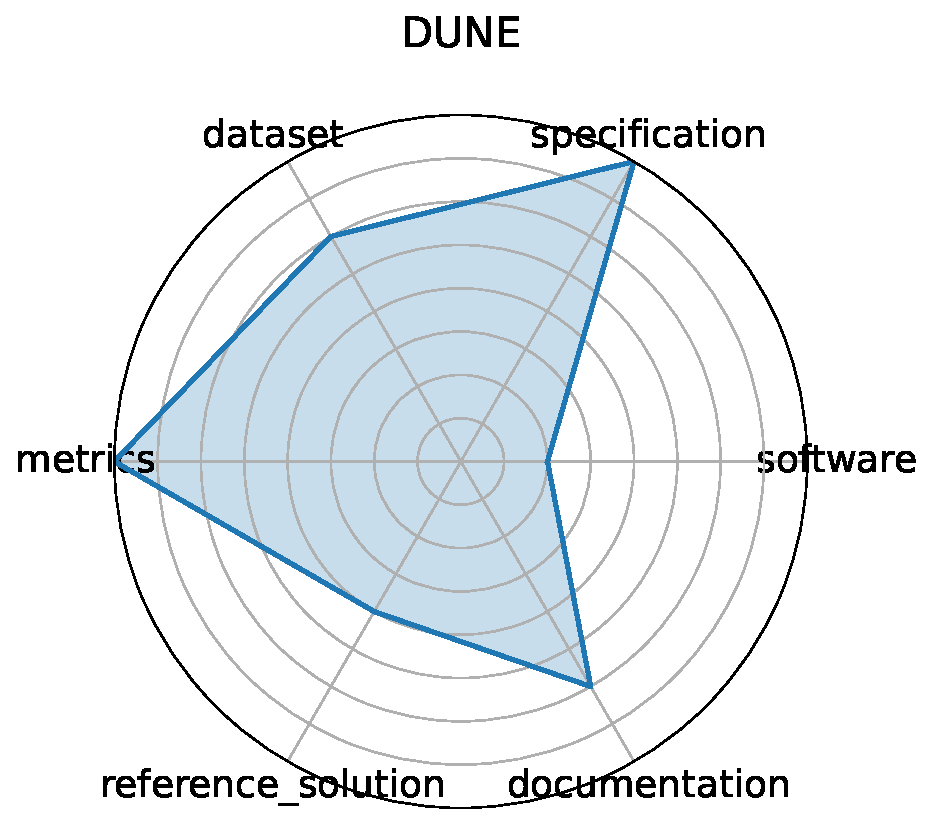
\includegraphics[width=0.2\textwidth]{dune_radar.pdf}
\end{description}
}}
\clearpage